\documentclass[11pt,a4paper]{article}
\usepackage[latin5]{inputenc}
\usepackage[english]{babel}
\usepackage{amsmath}
\usepackage{amsfonts}
\usepackage{amssymb}
\usepackage{graphicx,subfig}
\usepackage{placeins}
\author{Alexander Attinger, Yannic Kilcher}
\title{Report Blatt 2}

\begin{document}
\maketitle
\section{Exercise 1}
\subsection{a}
Since fourier transformed image consists of complex numbers, its magnitude and phase show the values of the phase and absolute length of these complex numbers. We've transformed the given image into the fourier domain (see Fig.\ref{fig:a1a}) and have displayed its phase and its magnitude specifically its \emph{log-magnitude}, since the magnitude image itself shows a single white dot in the middle of a black picture.
The phase image does not contain much interpretable information. The magnitude image, however, shows, which frequencies make up the original image in each direction. In our case, one can clearly see the diagonal line in the magnitude image, representing all the trigonometric functions that make up the striped pattern of the original image.

\begin{figure}%
\centering
\subfloat[][Original Image]{
\includegraphics[scale=.3]{res/striped-lines.png}}
\quad
\subfloat[][Phase Image]{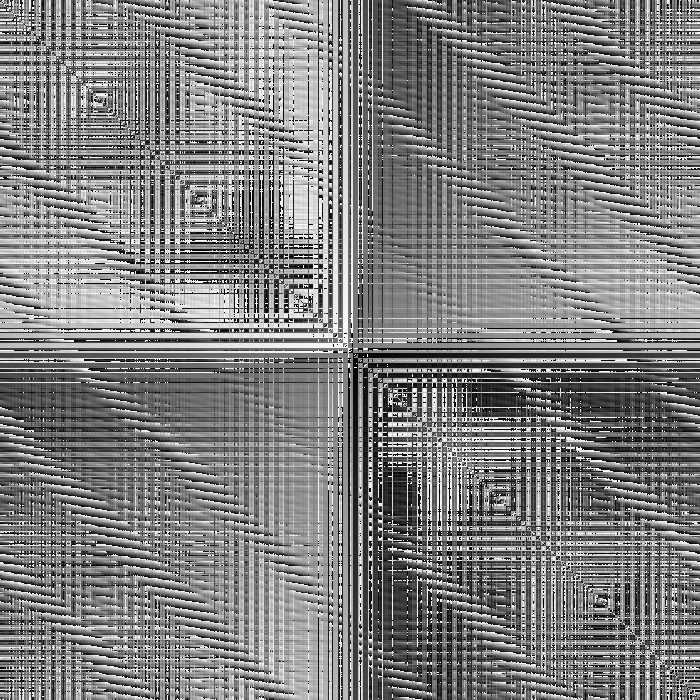
\includegraphics[scale=.3]{res/a1phase.png}}
\quad
\subfloat[][Log Magnitude Image]{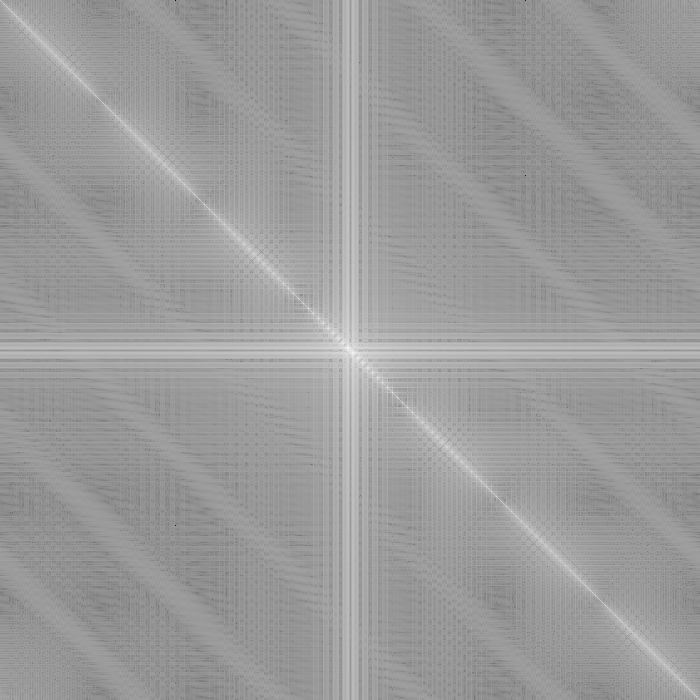
\includegraphics[scale=.3]{res/a1mag.png}}
\quad

\caption{Fourier transformation of a stripe pattern.}%
\label{fig:a1a}%
\end{figure}

\subsection{b}
We have convolved the two images in Fig.\ref{fig:a1b} and obtained the result image shown. Note the darker borders, where the convolution calculation includes pixels lying outside the source image, which are then valued 0.

\begin{figure}%
\centering
\subfloat[][Original Image 1]{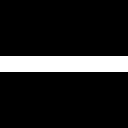
\includegraphics[scale=.7]{res/h.png}}
\quad
\subfloat[][Original Image 2]{
\includegraphics[scale=.7]{res/v.png}}
\quad
\subfloat[][Result after convolution]{
\includegraphics[scale=.7]{res/a2.png}}
\quad

\caption{Spatial convolution of two images.}%
\label{fig:a1b}%
\end{figure}

\subsection{c}
We have convolved the two images in Fig.\ref{fig:a1c}, but in the frequency domain. We have transformed both to the frequency domain, and then multiplied them element-wise. The result image can be obtained by transforming the outcome of the multiplication back to the spatial domain. Note that both methods of convolution produce the same result.
\begin{figure}%
\centering
\subfloat[][Original Image 1]{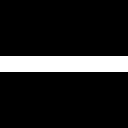
\includegraphics[scale=.7]{res/h.png}}
\quad
\subfloat[][Original Image 2]{
\includegraphics[scale=.7]{res/v.png}}
\quad
\subfloat[][Result after convolution]{
\includegraphics[scale=.7]{res/a3.png}}
\quad

\caption{Frequency convolution of two images.}%
\label{fig:a1c}%
\end{figure}

\FloatBarrier

\subsection{d}
We have done the previous two steps for higher resolutions of the same images and compared execution times of spatial and frequency convolution. Times in table \ref{tbl:t4} are measured in ms.
\begin{table}
\begin{tabular}{|l|r|r|}
imagesize&spatial domain&frequency domain\\\hline
128x128&0&0\\
1000x1000&280&80\\
10000x10000&68090&9540\\
\end{tabular}
\caption{Comparing spatial and frequency domain filtering speeds on differently resoluted images.}
\label{tbl:t4}
\end{table}
\\
Theoretically, the spatial convolution should be faster on small images, as the fourier transformation takes time, but slower on large images, as it is less efficient than the frequency convolution complexity-wise.
\end{document}
